\documentclass[a4paper,addpoints]{exam}

\usepackage{commath}
\usepackage{siunitx}

% russian integral
\usepackage{scalerel}
\DeclareMathOperator*{\rint}{\scalerel*{\rotatebox{17}{$\!\int\!$}}{\int}}

\qformat{\textbf{\large{Question \thequestion}}\hfill}
\pointsinrightmargin

\begin{document}

\begin{coverpages}

\begin{center}
  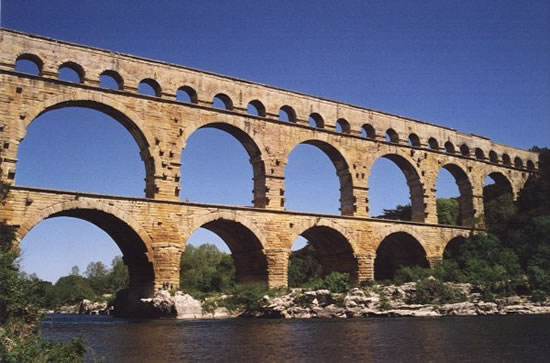
\includegraphics[width=0.6\textwidth]{exam-cover-01}

  \vspace{5mm}

  \textbf{\Huge{Level Three Calculus}}

  \vspace{2mm}

  \textbf{\Huge{Differentiation}}
\end{center}

\vspace{5mm}

\noindent
\large{There are three questions, worth a total of \numpoints\ marks.\\
       Attempt ALL questions, showing all working.\\
       Read questions carefully before attempting them.\\
       Marks are available for partial answers.\\
       The amount of time expected to be spent per question may not necessarily correlate ``nicely'' to the number of marks.\\
       Diagrams may be used to support answers.\\
       Candidates who do not provide diagrams for some questions may be disadvantaged.\\
       Some marks are given for clarity and neatness of solutions or proofs.}
\vspace{2mm}

\begin{tabular}{ll}
  \textbf{Time Allowed:}& One Hour\\
  \textbf{Achieved:}& 10 marks\\
  \textbf{Merit:}& 17 marks\\
  \textbf{Excellence:}& 24 marks
\end{tabular}

\vfill

\begin{center}
  \gradetable[h][questions]
  \vspace{2mm}

  \textbf{Available Grades:} \textit{Not Achieved}\quad\textit{Achieved}\quad\textit{Merit}\quad\textit{Excellence}
\end{center}

\end{coverpages}

\begin{questions}
  \question
    \begin{parts}
      \part[1] Differentiate
        \begin{displaymath}
          y = x^2 + x + 1 + \frac{1}{x} + \frac{1}{x^2}.
        \end{displaymath}
      \part[3] A stone is dropped into a lake. The resulting circular ripple spreads at a constant speed of
            \SI{0.5}{\metre\per\second}. Find the rate of change of the area of the ripple after 10 seconds.
      \part[4] Consider an equilateral triangle with side length $ L $. Find the maximum area of a rectangle
            sitting on the lowest edge of the triangle (as shown in figure \ref{fig:triangle}). \textit{You
            need not prove that you have found a maximum.}
            \begin{figure}
              \centering
              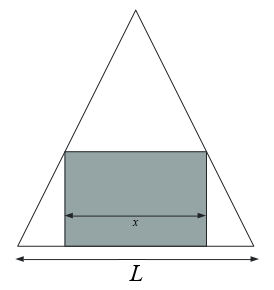
\includegraphics[width=0.3\textwidth]{triangle-optimisation}
              \caption{A triangle with an inscribed rectangle.\label{fig:triangle}}
            \end{figure}
    \end{parts}
  \question
    \begin{parts}
      \part Suppose $ f $ is a function defined by
            \begin{displaymath}
              f(x) = \cos (2x) + e^{x/2}.
            \end{displaymath}
        \begin{subparts}
          \subpart[2] Find $ f'(x) $ and $ f''(x) $.
          \subpart[1] Determine the nature of the critical point of $ f $ at $ (0, 0) $.
        \end{subparts}
      \part Consider the function $ g $ shown in figure \ref{fig:limits}.
            \begin{figure}
              \centering
              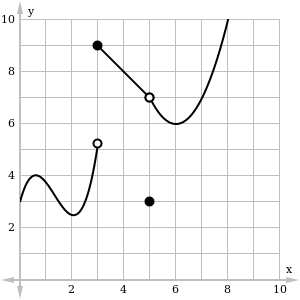
\includegraphics[width=0.35\textwidth]{limits1}
              \caption{The graph of $ y = g(x) $.\label{fig:limits}}
            \end{figure}
        \begin{subparts}
          \subpart[1] Find $ g(3) $.
          \subpart[2] Explain why $ \lim\limits_{x \to 3} g(x) $ does not exist.
          \subpart[1] Find the value of $ \lim\limits_{x \to 5} g(x) $.
        \end{subparts}
      \part[3] From first principles, prove that
            \begin{displaymath}
              \od{}{t} (x^2 - 5x) = 2x - 5.
            \end{displaymath}
    \end{parts}
  \question
    \begin{parts}
      \part[2] Find $ \od{x}{t} $ if
            \begin{displaymath}
              x = \frac{\sec t}{1 + \tan t}.
            \end{displaymath}
      \part A boat follows a parabolic trajectory determined by the parametric equations
            \begin{align*}
              y(t) &= 2t^2\\
              x(t) &= 4t
            \end{align*}
            and shown in figure \ref{fig:lighthouse}.

            \begin{figure}
              \centering
              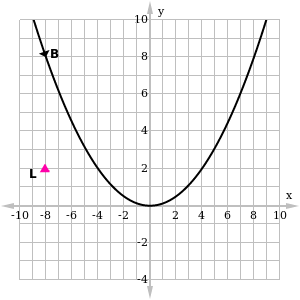
\includegraphics[width=0.35\textwidth]{lighthouse}
              \caption{The trajectory of a boat.\label{fig:lighthouse}}
            \end{figure}
        \begin{subparts}
          \subpart[2] Find $ \od{y}{x} $ in terms of $ x $ only.
          \subpart[4] For which value of $ t $ is the distance between the lighthouse $ L $ at $ (-8, 2) $ and the boat $ B $
                   at a minimum? \textit{You need not prove that the value which you find is a minimum.}
        \end{subparts}
      \part[2] Show that if
            \begin{displaymath}
              y = \frac{1}{m} \sec^2 (m \ln \theta)
            \end{displaymath}
            (where $ m $ is a constant) then the rate of change of $ y $ with respect to $ \theta $ when $ \theta = 1 $ is 0.
    \end{parts}
\end{questions}
\end{document}
